%!TEX encoding = UTF-8 Unicode
%!TEX root = ./../main.tex
%!TEX TS-program = xelatex

\chapter{Preliminari} % Main chapter title
\label{app:uno}
Lo scopo di quest'appendice è di stabilire una comune sintassi e semantica per concetti che sono rilevanti in tutta la tesi. Le definizioni e le notazioni qui introdotte sono essenziali per la maggior parte dei capitoli e quindi andrebbero lette.

L'appendice è divisa concettualmente in tre parti. Nella prima parte si introdurranno questioni  puramente matematiche mentre nella seconda parte si definiranno grammatiche e linguaggi, infine nell'ultima parte si tratteranno in dettaglio gli automi a stati finiti. 

\section{Notazione matematica}
L'obiettivo di questa sezione è di introdurre i concetti matematici propedeutici per questa tesi. Senza dubbio una conoscenza matematica di base è necessaria e chiaramente non può essere introdotto ogni singolo elementare concetto.
\subsection{Insiemi}
Con $\mathbb{N}$ si indica l'insieme di numeri naturali interi non negativi incluso 0 (cioè $\mathbb{N} = {0,1,2,\dots}$). L'insieme di interi positivi è denotato da $\mathbb{N}^{+}$ . Si definisce con $\mathbb{B} = \{0,1\}$ l'insieme di valori booleani dove 0 è associato al valore logico \textit{falso} ed 1 al valore logico \textit{vero}.

Dato un generico insieme $X, \abs{X}$ denota la sua cardinalità, cioè il numero di elementi che contiene.
\subsection{Relazione d'equivalenza}
Una relazione binaria riflessiva ,simmetrica e transitiva  $\approx \, \subseteq X\!\times{}\!X$ su un insieme $X$ è detta una \textbf{\textit{relazione d'equivalenza}}. Dato un insieme $X$ ed un elemento $x \in X$ si denota con $[x]_\approx = \{x' \in X\ | \: x \approx x'\}$ la \textit{classe di equivalenza} di x(rispetto alla relazione d'equivalenza $\approx$).

Una relazione d'equivalenza $\approx$ su un insieme \textit{X} si dice che \textit{satura} un sottoinsieme $X' \subseteq X$ se e solo se $X'$ è l'unione di alcune delle classi d'equivalenza di $\approx$. In simboli si ha:
\begin{equation*}
X' = \bigcup_{x \in X'}^{}{\!\![x]_\approx} \text{ ,}
\end{equation*}
e ogni classe di equivalenza $[x]_\approx \text{ di } \approx$ o è un sottoinsieme o è disgiunta da $X'$.\\
Il \textbf{\textit{quoziente}} (o insieme quoziente) di \textit{X} rispetto a una relazione d'equivalenza $\approx$ è definito come l'insieme di tutte le classi d'equivalenza, ed è indicato da $X\!/\!\!\approx  \:=  \{[x]_\approx \: | \: x \in X \}$. L'\textbf{\textit{indice di una relazione d'equivalenza}} $\approx$ è definito come il numero di classi d'equivalenza, cioè è uguale a $\abs{X\!/\!\!\approx}$ .
 Una \textit{partizione} di un insieme $X$ è un insieme $P$ i cui elementi, detti \textit{blocchi} ed indicati con $C$, sono sottoinsiemi (disgiunti e non vuoti) dell'insieme $X$ tali che: 
\begin{enumerate}
\item se $C \in P \text{ allora } C \ne \emptyset$
\item se $C_1,C_2 \in P \text{ e } C_1 \ne C_2 \text{ allora } C_1 \cap C_2  = \emptyset   $
\item se $a \in X \text{ allora esiste } C \in P \text{ tale che } a \in C$ (è un altro modo di dire che l'unione di tutti gli insiemi C deve formare X)
\end{enumerate}  
Il \textit{quoziente} di \textit{X} forma una \textit{partizione} di \textit{X}

\section{Linguaggi e grammatiche}
\subsection{Alfabeto, stringhe e linguaggi}
\subsubsection{Alfabeto}
Di definisce L'\textbf{\textit{alfabeto}} $\Sigma$ un qualsiasi insieme finito e non vuoto di simboli.

\subsubsection{Stringhe}
Una \textbf{\textit{stringa}} è definita come una sequenza di simboli presi da un alfabeto. Cioè una stringa \textit{s} definita su $\Sigma$ è una sequenza $ s = a_1\dots{}a_n$ tale che $a_i \in \Sigma$. 

$\abs{s}$ denota la lunghezza  della stringa s.\\
La \textit{stringa vuota} è indicata con $\epsilon$ e $\abs{\epsilon} = 0$. \\
Con $\Sigma^{*}$ si denota l'insieme di tutte le possibili stringhe ottenibili sull'alfabeto $\Sigma$. Inoltre con $\Sigma^{+}$ si denota l'insieme $\Sigma^{*} - \{\epsilon\}$ \\
I singoli simboli costituenti una stringa $w \in \Sigma^{*}$ sono indicati con $w_i$ con $0 \leq i \le \abs{w}$ quindi $w = w_0 w_1 \dots w_{\abs{w}-1}$ . Per qualche intero nell'intervallo $I \subseteq [0,\abs{w}], w_I$ è la stringa risultante prendendo solo le posizioni in w corrispondenti agli indici in $I$ . Quindi $w_{[0,k)}$ è il prefisso di w di lunghezza k, e $w_{[k,\abs{w})}$ è il suffisso di w che inizia all'indice k(compreso). Si osservi che $w_{[0,0)} = w_{[\abs{w},\abs{w})} = \epsilon$ e $w_{[0,\abs{w})} = w$ .\\
Un \textbf{\textit{prefisso}}  di una stringa $w \in \Sigma^{*}$ è una stringa $u \in \Sigma^{*}$ tale che esiste una stringa $v \in \Sigma^{*}$ soddisfacente $w=uv$. L'insieme di tutti i prefissi di una stringa $w$ si indica con Pref(w)\\
Un \textbf{\textit{suffisso}}  di una stringa $w \in \Sigma^{*}$ è una stringa $v \in \Sigma^{*}$ tale che esiste una stringa $u \in \Sigma^{*}$ soddisfacente $w=uv$. L'insieme di tutti i suffissi di una stringa $w$ si indica con Suff(w)\\
Una \textbf{sottosequenza} di una stringa è una qualsiasi stringa ottenuta rimuovendo dalla stringa di partenza zero o più simboli non necessariamente consecutivi.
\subsubsection{Linguaggi}
Un linguaggio \textit{L} su un alfabeto $\Sigma$ è un qualsiasi sottoinsieme di stringhe di $\Sigma^{*}$\\ 
Si definisce l'insieme dei prefissi di un linguaggio \textit{L}:
\begin{equation*}
 \text{Pref}(L) = \bigcup_{w \in L}^{}{\text{Pref}(w)}
 \end{equation*}
e l'insieme dei suffissi di \textit{L}:
\begin{equation*}
 \text{Suff}(L) = \bigcup_{w \in L}^{}{\text{Suff}(w)}
 \end{equation*}
 Un linguaggio \textit{L} è detto essere \textbf{\textit{prefix-closed}} se e solo se $\text{Pref}(L) = L$ . Informalmente questa proprietà di un linguaggio \textit{L} viene sfruttata per indicare che qualunque stringa appartenente ad \textit{L} si prende, qualunque suo prefisso deve ancora appartene ad \textit{L}. Analogamente un linguaggio \textit{L} è \textbf{\textit{suffix-closed}} se e solo se $\text{Suff}(L) = L$ . \\
 
 La \textbf{\textit{differenza simmetrica}} di due linguaggi $L_1 \text{ e } L_2$ denotata con $L_1 \oplus L_2$ è tale che:
 \begin{equation*}
 L_1 \oplus L_2 = \{x \in \Sigma^{*} : (x \in L_1 \land x \notin  L_2) \lor (x \notin L_1 \land x \in L_2)
 \end{equation*}
 Un linguaggio può essere identificato mediante due tipi di descrizioni:
 \begin{enumerate}
 \item \textbf{Descrizione generativa}\\Consiste nell'utilizzare un formalismo denominato \textbf{grammatica generativa} ,introdotto da Noam Chomsky, che consiste in una serie di simboli e regole mediante le quali è possibile generare tutte e sole le stringhe del linguaggio.
 \item \textbf{Descrizione descrittiva-identificativa}\\Il linguaggio è identificato o tramite un'enumerazione delle stringhe che vi appartengono o tramite una descrizione che cattura le caratteristiche delle sentenze costituenti il linguaggio,ad esempio le espressioni regolari. Un altro sistema formale identificativo sono gli \textbf{automi} .
 \end{enumerate}
 I linguaggi possono essere classificati in base ai due tipi di descrizioni.  Infatti è possibile delineare una tassonomia di grammatiche cui si farà corrispondere una classe di linguaggi. Ad ogni classe di grammatiche corrisponderà una classe di linguaggi (tutti quelli che quella classe di grammatiche è in grado di generare). 
E' possibile effettuare un'analoga corrispondenza tra classi di automi e classi di linguaggi, e quindi anche tra la gerarchia di automi e quella di grammatiche. Si rimanda alla sottosezione \ref{sub:gra} per una formalizzazione di questa gerarchia. 
 
 
 \subsection{Grammatiche}
 \label{sub:gra}
 \begin{definizione*}[Grammatica generativa di Chomsky] Una \textit{\textbf{grammatica generativa di Chomsky}} è una quadrupla:\\
 
 \centerline{$G = (\Sigma, V, S, P)$}
 

 dove:\\
 $\Sigma$ è l'alfabeto, detto insieme di simboli terminali\\
 V è l'insieme di simboli non terminali\\
 S è il simbolo iniziale ed appartiene a V\\
 P è l'insieme delle produzioni costituiti da una testa $\Psi$ (il lato sinistro della produzione) e da una coda $\Omega$ aventi in generale questa forma:\\

 \centerline{$\Psi \rightarrow \Omega \text{ con } \Psi \in (\Sigma \cup V)^{*}V(\Sigma \cup V)^{*} \text{ e } \Omega \in (\Sigma \cup V)^{*}$}
 \end{definizione*}
 Si effettua una classificazione delle classi di grammatiche (e dei linguaggi ad esse associate) imponendo delle restrizioni sulle regole di produzione \cite{Chomsky59}:
 \begin{itemize}
 \item \textbf{Grammatiche di tipo zero - Unresticted} E' la classe di grammatiche più in alto nella gerarchia e per la quale non vi sono regole di restrizione da applicare alle produzioni. Sono in grado di generare la classe di \textbf{linguaggi ricorsivamente enumerabili}. Mediante l'approccio identificativo l'automa che riconosce ed accetta questi linguaggi è la \textbf{Macchina di Turing}
 \item \textbf{Grammatiche di tipo uno - Context Sensitive} Le regole di produzione sono così definite:\\
 \centerline{$\alpha_1 A \alpha_2 \rightarrow \alpha_1 \Omega \alpha_2 \text{ con } \alpha_1 ,\alpha_2 ,\Omega \in (\Sigma \cup V)^{*} \text{ e } A \in V$}
 
  La classe di linguaggi che queste grammatiche sono in grado di generare è detta \textbf{context-sensitive}. Gli automi in grado di riconoscere ed identificare questi linguaggi sono detti \textbf{Linear Bounded Automata}
 \item \textbf{Grammatiche di tipo due - Context Free} Le regole di produzione sono così definite:\\
 \centerline{$A \rightarrow \Omega \text{ con } \Omega \in (\Sigma \cup V)^{*} \text{ e } A \in V$}
 
  La classe di linguaggi che queste grammatiche sono in grado di generare è detta \textbf{context-free}. Gli automi in grado di riconoscere ed identificare questi linguaggi sono detti \textbf{Push Down Automata}
 \item \textbf{Grammatiche di tipo tre - Regular} Le regole di produzione sono così definite:\\
 \centerline{$A \rightarrow \alpha B \text{ oppure } A \rightarrow B\alpha  \text{ con } A \in V, B \in (V \cup \{\epsilon\}) \text{ e } \alpha \in \Sigma^{+}$}
 
 I linguaggi che queste grammatiche generano sono detti \textbf{linguaggi regolari}. Gli automi in grado di riconoscere ed identificare questi linguaggi sono detti \textbf{\ac{FSA}}.    
 \end{itemize}
 
Le diverse classi di linguaggi, e quindi anche di grammatiche ed automi, si includono propriamente in maniera gerarchica come in figura \ref{fig:linger} .
\begin{figure}[htp]
	\centering
	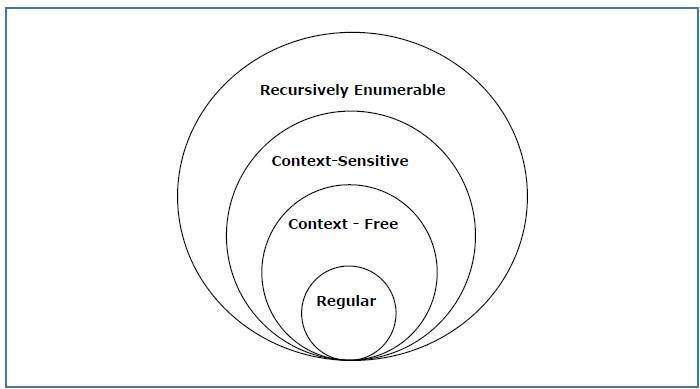
\includegraphics[ width=0.7\textwidth]{LinguaggiGerarchia}
	\caption[Gerarchia di linguaggi]{Gerarchia di linguaggi secondo Chomsky}
   \label{fig:linger}
\end{figure}
Ad una grammatica si può associare un unico linguaggio. Adesso si definirà come avvenie tale associazione:
\begin{definizione*}
Il linguaggio generato da una grammatica $\mathcal{G}$ è l'insieme di tutte le stringhe che possono essere derivate a partire dal simbolo iniziale S:\\

\centerline{$L(\mathcal{G}) = \{x \in \Sigma^{*} :S\xRightarrow[]{\mathcal{G}} x\}$}
\end{definizione*}
E' rilevante notare che come detto una grammatica genera un unico linguaggio ma un linguaggio può essere generato da molteplici grammatiche.\\
Inoltre la tassonomia di Chomsky non è esaustiva di tutti i linguaggi possibili, infatti esistono dei linguaggi che non sono ricorsivamente enumerabili cioè non c'è nessuna macchina di Turing che li riconosce.\\
Infine esistono altre classi di linguaggi che non sono incluse nella classificazione appena esposta e che saranno adoperate nel corso della trattazione:
\begin{definizione*}[Linguaggio Ricorsivo] Un linguaggio $L$ è detto \textbf{ricorsivo} se è decidibile cioè esiste una macchina di Turing $M$ che accetta ogni stringa in $x \in L$ e rigetta ogni stringa $x \not\in L$
\end{definizione*}
I linguaggi regolari e context-free sono ricorsivi. Esistono invece linguaggi context-sensitive non ricorsivi, cioè non ne sono un sottoinsieme \cite[p. 124]{Levelt08}. Tutti  i linguaggi ricorsivi sono ricorsivamente enumerabili (cioè sono linguaggi semidecidibili per i quali una stringa non appartenente al linguaggio può essere sia rigettata che andare in ciclo infinito rispetto a una macchina di Turing) ma non è sempre vero il viceversa.
\begin{definizione*}[Linguaggio primitivo ricorsivo]
Un linguaggio è \textbf{primitivo ricorsivo} quando la sua funzione caratteristica è primitiva ricorsiva.
\end{definizione*}
Il concetto di funzione caratteristica è spiegato nella sezione \ref{sec:FSA}. Invece una funzione primitiva ricorsiva è una funzione definita come una delle funzioni di base o combinando le funzioni di base con operazioni come composizione e ricorsione. Per una definizione formale si rimanda a \cite{Rob47}. I linguaggi primitivi ricorsivi sono un sottoinsieme dei linguaggi ricorsivi.
\begin{definizione*}[Linguaggi superfiniti]
La classe dei linguaggi superfiniti è tale se contiene tutti i linguaggi finiti ed almeno un linguaggio infinito.
\end{definizione*}
 
\section{Automi a stati finiti}
\label{sec:FSA}
Nella sottosezione \ref{sub:gra} sono stati introdotti gli automi e una loro classificazione. Qui ci si concentrerà sullo studio dei \ac{FSA} in relazione ai linguaggi regolari, la classe dei linguaggi a cui questa tesi è rivolta. Come visto gli \ac{FSA} sono un caso speciale di \textit{macchina di Turing} e più nello specifico un caso speciale di \ac{FSM} che in questa sede non interessa definire. Qui basterà dire che   una \ac{FSM} è un \textit{transiction system} costituita da un insieme finito di stati dove ogni transizione è innescata da un'azione tra un insieme finito di azioni (di solito denotato da $\Sigma$). Esistono diversi tipi di \ac{FSM} come le \textit{Mealy Machines} e gli \ac{FSA}. Tra gli \ac{FSA} si annoverano gli \ac{NFA} strettamente correlati ai \ac{DFA} su cui si focalizzerà l'attenzione.
\begin{definizione}[Automa a stati finiti deterministico]
\label{def:dfa}
Un \ac{DFA} A è una quintupla:\\

\centerline{$A = \Braket{\Sigma,Q^{A},q_{\epsilon}^{A},\delta^{A}, \mathbb{F}_{\mathbb{A}}^{A}}$}
\end{definizione}
dove:\\
$\Sigma$ è un alfabeto\\
$Q^{A}$ è un insieme finito di stati\\
$q_{\epsilon}^{A} \in Q^{A}$ talvolta indicato come $q_{\lambda}^{A}$ è lo stato iniziale\\
$\delta^{A} : Q^{A} \times \Sigma \to Q^{A} $ è la funzione di transizione\\
$\mathbb{F}_{\mathbb{A}}^{A} \subseteq Q^{A}$ è l'insieme degli stati accettanti\\

Inoltre nel corso della trattazione seguendo \cite[p. 72]{DeLaHiguera10} in alcuni casi è conveniente utilizzare anche un'altra definizione per i \ac{DFA} uguale a quella appena data ma comprendente anche un nuovo insieme $\mathbb{F}_{\mathbb{R}}^{A} \subseteq Q^{A}$ che è l'insieme degli stati rigettanti. Quando si parlerà di \ac{DFA} si farà sempre riferimento alla prima definizione,quella classica,  a meno che non è specificato o l'utilizzo della seconda definizione risulta tacitamente evidente dall'utilizzo dell'insieme $\mathbb{F}_{\mathbb{R}}^{A}$. Si indica con $\norma{A} = \abs{Q^{A}}$. 
Inoltre in molti frangenti è conveniente utilizzare (questo è un discorso che esula dalla definizione di un \ac{DFA}) una versione estesa della funzione di transizione a una stringa anzichè ad un solo simbolo dell'alfabeto. Si definisce allora $\hat{\delta}^{A} : Q^{A} \times \Sigma^{*} \to Q^{A}$ definendo induttivamente $\hat{\delta}^{A}(q,\epsilon) = q \text{ e } \hat{\delta}^{A}(q,aw) = \hat{\delta}^{A}(\delta^{A}(q,a),w) \text{ per } q \in Q^{A} \text{ e } aw \in \Sigma^{+} \text{ e } w \in \Sigma^{*}$. Per la funzione di transizione estesa nel corso della tesi sarà anche usata interscambiabilmente la definizione $A[w] = \hat{\delta}^{A}(q_{\epsilon}^{A},w)$ . Inoltre si estende quest'ultima notazione agli insiemi di stringhe: $W \subseteq \Sigma^{*} \text{ | } A[W] = \{A[w] : w \in W\}$ .\\
 
Una stringa \textit{x} è detta essere accettata da un \ac{DFA} \textit{A} se e solo se $\hat{\delta}^{A}(q_\epsilon,x) = q'$ tale che $q' \in \mathbb{F}_\mathbb{A}^{A}$ che significa che usando la funzione di transizione estesa $\hat{\delta}^{A}$ a partire dallo stato iniziale è possibile arrivare ad uno stato accettante.   Il linguaggio individuato da un \ac{DFA} A è allora:\\
\centerline{$L(A) = \{x \in \Sigma^{*} : \hat{\delta}^{A}(q_\epsilon,x) \in \mathbb{F}_\mathbb{A}^{A}\}$}

Una relazione analoga a quanto visto tra linguaggi e grammatiche sussiste tra linguaggi e \ac{DFA}: un \ac{DFA} induce un solo linguaggio regolare, ma ad un linguaggio regolare corrispondono più \ac{DFA}.

In molti contesti è utile rifersi alla \textit{funzione di output}  di un \ac{DFA} A, $\lambda^{A}$ come:\\\\
\centerline{$
\lambda^{A} : \Sigma^{*} \to \mathbb{B}, \quad \forall w \in \Sigma^{*}\quad\lambda^{A}(w) = \begin{cases}
1
& \text{se $w \in L(A)$} \\
0 & \text{altrimenti}\\
\end{cases}
$}\\\\
La \textit{funzione di output} è la \textit{funzione caratteristica} di L(A).Inoltre $\lambda^{A}$ appena definita sopra può essere vista come un caso particolare, per $q=q_\epsilon^{A}$, di $\lambda_{q}^{A}(w)$ che assume valore  1 se $ \hat{\delta}^A(q,w) \in \mathbb{F}_{\mathbb{A}}^{A}$ . Ancora, due \ac{DFA} ,A e A' , sono \textbf{equivalenti} denotato da $A \cong A'$, se loro hanno la stessa \text{funzione di output}, cioè se $\lambda^{A} = \lambda^{A'}$, cioè se indivividuano lo stesso linguaggio. Il concetto di equivalenza è rilevante anche tra gli stati dello stesso \ac{DFA} ed informalmente due stati sono equivalenti se non esiste nessuna stringa che li distingue, cioè che partendo da quei due stati porta a stati di arrivo che sono uno accettante e l'altro no.
\begin{definizione*}[Stati equivalenti]
Detto A essere un \ac{DFA}, e q e p $\in Q^{A}$ stati di A. q e p sono \textit{equivalenti} ,denotato da $q \equiv p$, se $\lambda_{q}^{A} = \lambda_{p}^{A}$
\end{definizione*}
Una stretta correlazione tra l'equivalenza di stati e l'equivalenza di \ac{DFA} è il seguente risultato: $A \cong A' \Leftrightarrow q_{\epsilon}^{A} \equiv q_{\epsilon}^{A'}$.
Un altro concetto importante è quello di \textit{isomorfismo} tra due DFA.
\begin{definizione*}[Isomorfismo di \ac{DFA}]
Detti A ed $\text{A}'$ due \ac{DFA} definiti su $\Sigma$. A ed $\text{A}'$ sono detti isomorfici se esiste un isomorfismo $f : Q^{A} \to Q^{A'}$, cioè una funzione soddisfacente le seguenti condizioni:
\begin{enumerate}
\item $f(q_{\epsilon}^{A}) = q_{\epsilon}^{A'}$
\item $\forall q \in Q^{A} : q \in F_{\mathbb{A}}^{A} \Leftrightarrow f(q) \in F_{\mathbb{A}}^{A'}$
\item $\forall q \in Q^{A}, a \in \Sigma : f(\delta^{A}(q,a)) = \delta^{A'}(f(q),a)$
\end{enumerate} 
\end{definizione*}
L'isomorfismo è un requisito più forte dell'equivalenza: \ac{DFA} isomorfi sono pure equivalenti, ma in generale non è vero il contrario. Quindi dato un linguaggio L esistono più \ac{DFA} in grado di riconoscerlo cioè con la stessa \textit{funzione di output} $\lambda$. Tra questi di particolare interesse sono quelli con il minor numero di stati. Un \ac{DFA} A è detto \textbf{minimo} se qualunque altro \ac{DFA} $\text{A}'$ tale che $A \cong A'$ (con la stessa \textit{funzione di output}) soddisfa $\abs{Q^{A'}}\geq\abs{Q^{A}}$. Ovviamente in un \ac{DFA} minimo nè stati irragiungibili ne stati equivalenti possono essere presenti perchè potrebbero essere eliminati senza cambiare la funzione di output $\lambda$. Inoltre il DFA minimo è sempre unico a meno di una possibile rinomina degli stati. Per motivi storici esiste anche la definizione di \ac{DFA} \textbf{canonico} che è intercambiabile con quella di \ac{DFA} minimo ma entrambe indicano lo stesso ente matematico e sono del tutto equivalenti. Formalizzando
\begin{definizione*}[DFA minimo/canonico]
Detto A essere un \ac{DFA} su $\Sigma$. A è detto canonico se le seguenti condizioni sono verificate:
\begin{enumerate}
\item Tutti gli stati sono raggiungibili: $A[\Sigma^{*}] = Q^{A}$
\item Tutti gli stati sono a coppie separabili\footnote{due stati sono separabili o distinti se non sono equivalenti}: $\forall q \ne p \in Q^{A} : \exists w \in  \Sigma^{*} : \lambda_{q}^{A}(w) \ne \lambda_{p}^{A}(w)$
\end{enumerate}
\end{definizione*}
Per ogni DFA esiste sempre ,ed è unico (a meno delle etichette degli stati) un \ac{DFA} equivalente  che è canonico.
\subsection{FSA particolari}
Alcuni \ac{DFA} ed \ac{NFA} sono particolarmente significativi e ricorreranno spesso nell'ambito di questa tesi. Inoltre è necessario conoscere per il proseguio della trattazione qual è la differenza principale tra \ac{DFA} ed \ac{NFA}. Un \ac{NFA} è detto non deterministico perchè la sua funzione di transizione può avere più di una transizione per un dato simbolo dell'alfabeto (ed inoltre vi possono essere transizioni anche in corrispondenza di $\epsilon$). Inoltre in un \ac{NFA} non vi è necessariamente per ogni stato una transizione in corrispondenza di ogni simbolo dell'alfabeto.
\subsubsection{Maximal Canonical Automaton}
\begin{definizione}[Maximal Canonical Automaton]
Detto $I_+ = \{x_1,\cdots ,x_N\}$ un insieme di esempi positivi, si definisce \textit{\textbf{Maximal Canonical Automaton rispetto ad $I_+$}} e si denota con \textit{\textbf{MCA($I_+$)}} un \ac{NFA} costituito da una quintupla $\Braket{\Sigma , Q , q_\epsilon , \delta , \mathbb{F}_\mathbb{A}}$ dove:\\\\
$\Sigma$ è l'alfabeto su cui è definito $I_+$\\
$Q = \{q_{u}^{i} : u \in \text{Pref}(x_i) \land u \ne \epsilon \} \cup \{q_\epsilon\}, 1 \leq i \leq N$\\
$q_\epsilon = \{q_\epsilon\}$\\
$\delta(q_{u}^{i},a) = \{q_{ua}^{i} : ua \in \text{Pref}(x_i)\}, \forall a \in \Sigma, 1 \leq i \leq N$\\
$\delta(q_\epsilon,a) = \{q_{a}^{i} : a \in \text{Pref}(x_i)\}, \forall a \in \Sigma, 1 \leq i \leq N$\\
$1 \leq i \leq N, q_{x_{i}}^{i} \in \mathbb{F}_\mathbb{A} $\\
se $\epsilon \in I_+$ aggiungere $q_\epsilon \text{ ad } \mathbb{F}_\mathbb{A}$
\end{definizione}
Un \textit{MCA($I_+$)} per ogni stringa di $I_+$ ha un percorso dedicato a partire dallo stato iniziale.
Si noti che nella definizione data di $\delta$ accade che per molti simboli di $\Sigma$ non c'è la corrispondente transizione per un dato stato. Inoltre se in $I_+$ sono presenti stringhe che hanno lo stesso simbolo iniziale si avrà indeterminismo sullo stato iniziale $q_\epsilon$. Quindi in generale il \textit{MCA($I_+$)} è un \ac{NFA}.Un esempio è dato in figura \ref{fig:MCA}\\\\
\begin{figure}
\centering
\begin{tikzpicture}[shorten >=1pt,node distance=2cm,on grid,auto] 
   \node[state,initial] (q_0)   {$\varepsilon$}; 
   \node[state] (q_1) [above right=of q_0] {$a$}; 
   \node[state] (q_2) [below right=of q_0] {$a$}; 
   \node[state] (q_3) [right=of q_1] {$p$};
   \node[state,accepting] (q_4) [right=of q_3] {$e$};
   \node[state](q_5) [right=of q_2] {$t$};
   \node[state](q_6) [right=of q_5] {$o$};
    \node[state](q_7) [right=of q_6] {$l$};
    \node[state](q_8) [right=of q_7] {$l$};
    \node[state,accepting](q_9) [right=of q_8] {$o$};
    \path[->] 
    (q_0) edge  node {$a$} (q_1)
           edge  node {$a$} (q_2)
    (q_1) edge  node  {$p$} (q_3)
    (q_3) edge  node  {$e$} (q_4)
    (q_2) edge  node  {$t$} (q_5)
    (q_5) edge  node  {$o$} (q_6) 
    (q_6) edge  node  {$l$} (q_7)
    (q_7) edge  node  {$l$} (q_8) 
    (q_8) edge  node  {$o$} (q_9); 
\end{tikzpicture}
\caption[Maximal Canonical Automaton]{\textit{MCA($I_+$)} per $I_+=\{\text{ape,atollo}\}$}
\label{fig:MCA}
\end{figure}

\subsubsection{Automa quoziente}
\label{subsub:aqu}
Sia A un \ac{DFA} su $\Sigma$ e sia  $\approx \: \subseteq Q^{A}\!\!\times{}\!Q^{A}$ una relazione d'equivalenza sull'insieme $Q^{A}$ soddisfacente le seguenti due condizioni:
\begin{enumerate}[label=(\roman*)]
\item $\approx$ satura $\mathbb{F}_{\mathbb{A}}^{A}$
\item $\forall q,p \in Q^{A} : q \approx p \Rightarrow (\forall a \in \Sigma : \delta^{A}(q,a) \approx \delta^{A}(p,a) )$ 
\end{enumerate}
Allora da A tramite $\approx$ è possibile ricavare il \textit{\textbf{DFA quoziente}} \textbf{$A/\!\!\approx$} così definito:
\begin{enumerate}
\item $\Sigma$ è lo stesso di $A$
\item $Q^{A/\!\approx} = Q^{A}/\!\!\approx$
\item $q_\epsilon^{A/\!\approx} = [q_\epsilon^{A}]_\approx$
\item $\mathbb{F}_\mathbb{A}^{A/\!\approx} = \{[q]_\approx : q \in \mathbb{F}_\mathbb{A}^{A}\}$
\item $\delta^{A/\!\approx}([q]_\approx,a) = [\delta^{A}(q,a)]_\approx \quad \forall q \in Q^{A},a\in{\Sigma}$
\end{enumerate}
L'automa quoziente $A/\!\!\equiv$ ,dove la relazione d'equivalenza utilizzata è quella di equivalenza tra gli stati, corrisponde al \ac{DFA} canonico. Quindi banalizzando si può concludere dicendo che l'automa quoziente di un \ac{DFA} è ciò che si ottiene fondendo insieme alcuni stati del \ac{DFA} di partenza in base a una relazione d'equivalenza. Quando la relazione usata è quella di stati equivalenti si ottiene il DFA minimo: quindi $Q^{A/\!\approx}$ sarà una partizione in cui in ogni blocco (sottoinsieme) ci saranno stati equivalenti tra loro (in uno specifico blocco). Ogni blocco è una classe d'equivalenza.

\subsubsection{Prefix Tree Acceptor}
Si è visto che l'automa quoziente che si ottiene usando la relazione di equivalenza degli stati su un \ac{DFA} A è il \ac{DFA} minimo. Analogamente è possibile ottenere il \textit{\textbf{Prefix Tree Acceptor di $I_+$}} indicato con \textit{\textbf{PTA$(I_+)$}} applicando la definizione di automa quoziente al \textit{MCA$(I_+)$}\footnote{Anche se tecnicamente può essere un \ac{NFA} la definizione di automa quoziente può essere applicata comunque} con la relazione: \textit{stati che identificano lo stesso prefisso}. Quindi verrà effettuata la fusione degli stati che condividono lo stesso prefisso.\\
Si definisce la relazione d'equivalenza come:
\begin{equation*}
p \approx q \Leftrightarrow \text{ Prefix}(p) = \text{ Prefix}(q)
\end{equation*}
allora:
\begin{equation*}
MCA(I_+)/\!\!\approx \,\,=\, PTA(I_+)
\end{equation*}
In figura \ref{fig:PTA} il \textit{PTA} ricavato a partite dal \textit{MCA} di figura \ref{fig:MCA} .
\begin{figure}[htp]
\centering
\begin{tikzpicture}[shorten >=1pt,node distance=2cm,on grid,auto] 
   \node[state,initial] (q_0)   {$\varepsilon$}; 
   \node[state] (q_1) [right=of q_0] {$a$}; 
   \node[state] (q_3) [right=of q_1] {$p$};
   \node[state,accepting] (q_4) [right=of q_3] {$e$};
   \node[state](q_5) [below right=of q_1] {$t$};
   \node[state](q_6) [right=of q_5] {$o$};
    \node[state](q_7) [right=of q_6] {$l$};
    \node[state](q_8) [right=of q_7] {$l$};
    \node[state,accepting](q_9) [right=of q_8] {$o$};
    \path[->] 
    (q_0) edge  node {$a$} (q_1)
    (q_1) edge  node  {$p$} (q_3)
               edge  node  {$t$} (q_5)
    (q_3) edge  node  {$e$} (q_4)
    (q_5) edge  node  {$o$} (q_6) 
    (q_6) edge  node  {$l$} (q_7)
    (q_7) edge  node  {$l$} (q_8) 
    (q_8) edge  node  {$o$} (q_9); 
\end{tikzpicture}
\caption[Prefix Tre Acceptor]{\textit{PTA($I_+$)} per $I_+=\{\text{ape,atollo}\}$}
\label{fig:PTA}
\end{figure}

\subsubsection{Automa Universale}
Si indica con \textit{\textbf{UA l'automa universale}} che accetta tutte le stringhe definite su $\Sigma$. Si ha $L(UA) = \Sigma^{*}$. Ha un unico stato,che è accettante, con un \textit{self-loop} per ogni simbolo dell'alfabeto.

\subsection{Funzioni di output regolari}
In una sottosezione di \ref{subsub:aqu}  si è visto che è possibile ottenere il  \ac{DFA} canonico minimo di un \ac{DFA} A tramite $A/\!\!\equiv$ (l'automa quoziente sulla relazione di stati equivalenti). In questa sezione invece si vedrà come ottenere il \ac{DFA} canonico minimo non a partire da un \ac{DFA} preesistente, ma semplicemente sfruttando le proprietà di una funzione di output $\lambda : \Sigma^{*} \to \mathbb{B}$ che è la funzione caratteristica di qualche linguaggio regolare.
\subsubsection{Relazione di Nerode}
Si possono caratterizzare le \textit{funzioni di output regolare} come la classe di funzioni $\lambda : \Sigma^{*} \to \mathbb{B}$ per cui un \ac{DFA} con quella \textit{funzione di output} esiste\footnote{L'insieme delle funzione di output regolari identifica la classe dei linguaggi regolari}.  Il famoso teorema \textit{Myhill-Nerode} \cite{Ner58} fornisce una caratterizzazione alternative delle \textit{funzioni di output regolari} , che non fa affidamento sulla nozione di \ac{DFA}. Come primo step si definisce la \textit{relazione di Nerode} \cite{Ner58} sulle stringhe che definisce un'equivalenza sulle stringhe secondo $\lambda$:
\begin{definizione}[Relazione di Nerode]
\label{def:ner}
Sia $\lambda : \Sigma^{*} \to \mathbb{B}$ una funzione di output a due valori arbitraria definita su $\Sigma$. Due stringhe $u, u' \in \Sigma^{*}$ sono equivalenti secondo $\simeq_\lambda$\footnote{Si noti che per denotare l'equivalenza non si è usato il simbolo $\equiv$ (equivalenza tra stati) perchè qui si parla di equivalenza tra stringhe} denotato da $u \simeq_\lambda \!u'$ se e solo se:
\begin{equation*}
\forall v \in \Sigma^{*} \quad \lambda(uv) = \lambda(u'v)
\end{equation*}
dove $\simeq_\lambda \, \subseteq \Sigma^{*}\!\!\!\times\!\!\Sigma^{*}$ è una relazione binaria detta \textit{relazione di Nerode} o \textit{congruenza di Nerode} che definisce l'equivalenza tra stringhe secondo $\lambda$
\end{definizione}
\subsubsection{Teorema Myhill-Nerode}
La \textit{relazione di Nerode} $\simeq_\lambda$ può essere vista come l'equivalente a livello di stringhe della relazione di equivalenza $\equiv_A \subseteq Q^{A}\!\!\times\!Q^{A}$, sugli stati di un \ac{DFA} A. Dovrebbe essere osservato, tuttavia , che $\simeq_\lambda$ può essere definito per \textit{funzioni di output} arbitrarie, non solo regolari. Il teorema \textit{Myhill-Nerode}  fornisce una caratterizzazione delle \textit{funzioni di output regolari} basata su  $\simeq_\lambda$ :
\begin{teorema}[Teorema Myhill-Nerode o di caratterizzazione]
\label{teo:m-n}
Sia $\lambda : \Sigma^{*} \to \mathbb{B}$ una \textit{funzione di output} a due valori. $\lambda$ è regolare se e solo se la \textit{relazione di Nerode}  $\simeq_\lambda$ ha indice finito. 
\end{teorema}
Una dimostrazione del teorema si trova in \cite{Stef11}. L'implicazione in uno dei due versi del teorema dice che se $\simeq_\lambda$ ha indice finito, allora $\lambda$ è \textit{una funzione di output regolare} cioè esiste un \ac{DFA} A con $\lambda^{A} = \lambda$. Questo \ac{DFA} $A = \Braket{\Sigma,Q^{A},q_{\epsilon}^{A},\delta^{A},F_{\mathbb{A}}^{A}}$ è definito come:
\begin{itemize}
\item $\Sigma \text{ è il dominio di } \lambda$
\item $Q^{A} = \Sigma^{*}/\!\!\simeq_{\lambda}$
\item $q_{\epsilon}^{A} = [\epsilon]_{\simeq_{\lambda}}$
\item $F_{\mathbb{A}}^{A} = \{[u]_{\simeq_{\lambda}} | \: \lambda(u)=1\}$
\item $\delta^{A}([u]_{\simeq_{\lambda}} , a) = [u\!\cdot{}\!a]_{\simeq_{\lambda}}$ 
\end{itemize}
A è il \ac{DFA} minimo corrispondente al linguaggio identificato da $\lambda$.Si osservi come la costruzione del \ac{DFA} A è molto simile alla costruzione del \ac{DFA} minimo  usando la relazione di equivalenza sugli stati $\equiv$ usando l'automa quoziente a partire da un \ac{DFA}. Questo approccio alla costruzione degli automi è fondamentale nell'\textit{active learning}.

\chapter[Prel. e impl. ObP]{Preliminari e implementazione dell'Observation Pack}
\label{app:due}
Qui si presentano delle ulteriori notazioni inerenti prevalentemente il capitolo \ref{cap:quattro} e vengono svelati alcuni dettagli implementativi dell'\ac{ObP}.
\section{Notazione specifica per l'ObP}
In questo sezione vi è la delineazione di un'ulteriore notazione utilizzata principalmente nel capitolo \ref{cap:quattro} in congiunzione a quella introdotta in \ref{app:uno}, ma che essendo specifica dell'\ac{ObP} viene presentata in quest'appendice. Inoltre vi è anche la presentazione della notazione utilizzata per presentare un framework introdotto in \cite{StefCounterexample14} che facilità la compresione della correttezza e l'implentazione del metodo di gestione del controesempio in \ac{ObP}.
\subsection{Definizioni}
L'\ac{ObP} mantiene un insieme Sp,\textit{prefix-closed}, di \textbf{short prefix} detti anche \textbf{access sequence} ,che sono prefissi . Ogni short prefix identifica unicamente (cioè short prefix diversi identificano stati diversi in \ac{H} e nel target)  gli stati sia nel target A che nell'ipotesi \ac{H}. Ogni stato $q \in Q^{H}$ corrisponde unicamente ad una stringa (lo short prefix) $u \in Sp$, ed è assicurato che $H[u] = q$.  u è detta l'access sequence di q (in \ac{H}), ed è denotata da $\lfloor q \rfloor_{H}$ . Alternativamente quanto detto può essere formulato come $\forall q \in Q^{H} : \text{ \ac{H}}[\lfloor q \rfloor_{H}]=q$. Lo stato iniziale $q_{\epsilon}^{H}$ è lo stato con access sequence $\epsilon$.

Si estende questa notazione a stringhe arbitrarie $w \in \Sigma^{*} : \lfloor w \rfloor_{H} = \lfloor H[w] \rfloor_{H}$ che significa che w raggiunge uno stato in \ac{H} e questo stato ha un access sequence u cui w si associa. Quindi la funzione $\lfloor \cdot \rfloor_{H} : \Sigma^{*} \to Sp$ trasforma stringhe in access sequences.\\
Uno short prefix $u \in Sp$ corrisponde ad uno stato in A, cioè $A[u]$. Ci si riferisce ad $A[Sp]$ come gli stati scoperti (dal \textit{learner}) di A. Gli short prefixes quindi stabiliscono una funzione $f_{Sp}$ che collega stati nell'ipotesi e stati scoperti nel \ac{DFA} target A come segue:
\begin{equation*}
f_{Sp} : Q^{H} \to Q^{A} , f_{Sp}(q)=A[\lfloor q \rfloor_{H}]
\end{equation*}
\begin{comment}
Infine ,detto N l'insieme di nodi di un albero binario $\Upsilon$,si denota con o-child(n) la funzione d'utilità definita attraverso la funzione child(o,n) nella seguente maniera :
\begin{equation*}
\begin{multlined}
o-child=child : \mathbb{B} \times N  \to \{nil\} \cup N, \\
child(o,n)=\begin{cases}
n' & \parbox[t]{.6\textwidth}{se o=1 e n' è il figlio destro di n in $\Upsilon$ oppure o=0 e n' è il figlio sinistro di n in $\Upsilon$}\\
nil & \parbox[t]{.6\textwidth}{se o=1 e n non ha figli destri in $\Upsilon$ oppure o=0 e n non ha figli sinistri in $\Upsilon$}\\
\end{cases}
\end{multlined}
\end{equation*}
\end{comment}

%\thispagestyle{empty}

\subsection[Def. fram.]{Definizioni per il framework}
\label{sub:fra}
\subsubsection{Prefix Transformation}
\textit{Prefix transformation} è una procedura che consente di trasformare un prefisso di un controesempio $w \in \Sigma^{+}$ in un access sequence in Sp.
\begin{definizione*}[Prefix Transformation]
Prefix transformation rispetto ad \ac{H}, $\pi_{H}$ , è definita come segue:
\begin{equation*}
\pi_{H} : \Sigma^{*} \times \mathbb{N} \to \Sigma^{*} \text{ , } \pi_{H}(w,i) = \lfloor w_{[0,i)} \rfloor_{H} \cdot w_{[i,\abs{w})}
\end{equation*}
\end{definizione*}
Si osservi che, $\pi_{H}(w,0)=w \text{ e } \pi_{H}(w,\abs{w})=\lfloor w \rfloor_{H} \in Sp$.

\subsubsection{Altre definizioni}
Sia $w \in \Sigma^{+}$\footnote{In\ac{ObP} $\epsilon$ non può essere un controesempio} un controesempio che differenzia il target A da \ac{H}. Sia $m = \abs{w}$ ed i un indice $0\leq i \leq m$ allora si definisce la funzione $\alpha$ come:
\begin{equation*}
\alpha: [0,m+1) \to \mathbb{B}, \: \alpha(i) = \begin{cases}
1
& \text{se } \lambda^{A}(\pi_{H}(w,i)) = \lambda^{H}(w) \\
0 & \text{altrimenti}\\
\end{cases}\\\\
\end{equation*}
Dalla funzione $\alpha$ può essere ricavato anche la definizione della funzione $\beta$:
\begin{equation*}
\label{equ:beta}
\beta: [0,m) \to \{0,1,2\}, \: \beta(i) = \alpha(i) + \alpha(i+1)
\end{equation*}
\section[Dett. impl. ObP]{Dettagli implementativi dell' ObP}
\label{sec:implobp} 
Vengono ora riportati alcuni dettagli implementativi ritenuti più significativi senza pretesa di esaustività.
Per la memorizzazione della funzione OT (definizione \ref{def:obstable}) di un componente si è utilizzata una map che tipicamente è nella forma chiave-valore dove nella fattispecie la chiave è una stringa (ottenuta dalla concatenazione di un prefisso con un suffisso) ed il valore è l'esito delle \ac{MQ} nel target per quella stringa. Qui si è utilizzato per il valore un doppio campo oltre all'esito della \ac{MQ} costituito da un contatore del numero di volte che quella stringa viene a formarsi in un dato componente (una stessa stringa può essere formata da  coppie prefisso-suffisso diverse). Questo è dovuto al fatto che quando si effettua uno split di un componente alcuni dei prefissi del componente migrano nei prefissi del nuovo componente. Oltre all'insieme dei prefissi del componente splittato (che va decrementato) si può modificare anche il dominio della funzione OT restringendolo. Nel codice si è scelto di eliminare la concatenazione del prefisso che migra nel nuovo componente con l'insieme di suffissi del componente splittato, restringendo il dominio di OT. Tuttavia per garantire la correttezza è necessario appurare se quella concatenazione di quel prefisso con un dato suffisso si venga a formare anche tramite altri prefissi perchè in questo caso l'eliminazione non deve avvenire ed è per questo motivo che si usa un contatore per ogni stringa (per ogni concatenazione) che va incrementato ad ogni inserimento di una stringa (anche una già esistente) e decrementato nel caso suddetto.  Questa scelta è stata fatta nell'ottica di consentire velocemente di appurare se un componente è chiuso e in generale consentire una ricerca molto veloce di un prefisso in un componente. L'alternativa sarebbe stata quella di non utilizzare il contatore e non eliminare mai la stringa formata dalla concatenazione di un prefisso e di un suffisso ma solo il prefisso dal componente splittato. Ciò porterebbe ad una crescita del dominio di ricerca per la funzione OT che degraderebbe le prestazioni della ricerca di un prefisso in un componente (operazione effettuata sovente) anche se potrebbe  comportare una diminuizione del numero delle \ac{MQ} e l'eliminazione dell'\textit{overhead} per tenere aggiornato il contatore: questa prospettata diminuizione delle \ac{MQ} con questa seconda scelta è però possibile soltanto se quando si completano le componenti, ad esempio nella funzione UPDATE-FROM-COUNTEREXAMPLE  prima di effettuare una \ac{MQ} su una stringa x si controlli se per x non si conosca già l'esito della \ac{MQ} perchè contenuto già nel dominio della funzione OT\footnote{più è grande il dominio e maggiore sarà la probabilità di ottenere un \textit{hit} per x} anche se nel caso vi fossero molti \textit{miss} questa politica potrebbe essere addirittura controproducente. Anche quest'ulteriore strategia non è stata implementata ritenendo poco probabile un \textit{hit} (per implementarla basta decommentare un if  in UPDATE-FROM-COUNTEREXAMPLE e aggiungerne un altro nella funzione \textit{sift}). Se si fossero fatte delle scelte opposte a quelle fatte e appena descritte senz altro si sarebbe potuto abbassare ulteriormente il numero di \ac{MQ} ma si è ritenuto che il gioco non vale la candela cioè che il prezzo da pagare in termini di tempo di esecuzione per ottenere ciò è maggiore del beneficio ottenuto.\\
Si sottolinea che diversamente dal metodo OBP-SPLIT (algoritmo \ref{alg:split}) non viene ritornato il nuovo componente ottenuto perchè il chiamante OBP-CLOSEPACK ne è già a conoscenza , quindi il metodo non ritorna niente.\\
Infine si prende in esame l'implementazione del discrimination tree. Per quest ultimo si è scelto di usare un \textit{vector} di nodi e un insieme di archi. Per ogni nodo si memorizza l'etichetta e se è accettante o meno. Gli archi sono un \textit{vector} di array bidimensionali. L' indice di un nodo nel \textit{vector} di nodi è usato per accedere alla posizione nel \textit{vector} di archi che contiene gli indici dei nodi figli (nell'array contenuto nel \textit{vector} di nodi nella posizione individuata dall'indice del nodo). L'utilizzo di un insieme di nodi e di archi è tipico di un grafo piuttosto che di un albero binario. Si è scelta ugualmente questa implementazione essenzialmente per due ragioni:
\begin{itemize}
\item La \textit{Standard Template Library} non mette a disposizione nessuna struttura dati per modellare una albero binario. Esistono delle librerie esterne che mettono a disposizioni un albero n-ario ma l'overhead per gestire n figli ed altre operazioni inutili ai fini dell'\ac{ObP} ha fatto propendere per il declinare il loro utilizzo. Un'altra possibilità sarebbe stata quella d'implementare un albero binario \textit{ad hoc} nella maniera classica cioè tramite i puntatori ma essendo le prestazioni simili a quelle della soluzione adottata e descritta sopra non lo si è fatto. Inoltre si è supposto che chiamare un oggetto di una classe esterna (quella dell'eventuale implementazione dell'albero binario), dato che va fatto molte volte, sarebbe divenuto il costo preponderante. Il vantaggio principale nell'usare l'implementazione di un albero binario con i puntatori per il discrimination tree sta nel risparmio di memoria circa doppia ma comunque sempre lineare nella soluzione proposta, e che non avviene mai la riallocazione (operazione che accade quando le dimensioni del vettore superano la capacità dello stesso).
\item Utilizzare un vettore indicizzato. Questa soluzione è da scartare perchè se il discrimination tree non è bilanciato e presenta un ramo molto più lungo degli altri sarebbe necessario rendere il vettore molto grande. Il vettore può crescere dinamicamente ed è molto più probabile con un vettore indicizzato superare la capacità totale del vettore (se l'inserimento del nodo avviene nello stesso ramo ciò avviene molto velocemente) che verrebbe quindi riallocato e ricopiato frequentemente degradando le prestazioni.
\end{itemize} 
 
 \chapter[Prel. add.  class.]{Conoscenze preliminari nell'addestramento dei classificatori}
\label{app:due}
Questa appendice è propedeutica al capitolo \ref{cap:sei} e descrive succintamente alcune tecniche basilari di \textit{machine learning}  nell'addestramento dei classificatori che saranno impiegate per la costruzione del classificatore che approssima un \textit{Oracolo}. La trattazione non sarà esaustiva ma volta al fine di fare chiarezza su alcune delle scelte effettuate nel costruire l'\textit{Oracolo approssimato}. Per comprendere appieno quest'appendice è consigliabile leggere prima il capitolo \ref{cap:cinque}.

\section{Bias-Varianza tradeoff}
I concetti di modello,classificatore,classificazione,\textit{training set} e \textit{test set} sono stati introdotti nel \ref{cap:cinque}. In breve,  {eq:effe}il compito di un modello è quello di selezionare la funzione tra la famiglia di funzioni $\{f(x,\alpha)\}$ che da migliori garanzie di predire dati mai visti. Dati $X=x_1,\dots,x_l$ e le relative etichette $Y=y_1,\dots,y_l$ si assume che c'è qualche relazione tra i due insiemi che può essere espressa come:
\begin{equation}
Y = f(X) + \epsilon
\end{equation}
dove $\epsilon$ è un errore casuale a media zero, detto errore irriducibile.
$f(\cdot)$ è funzione ignota che rappresenta il mapping corretto tra ingressi ed etichette ed è necessario scovare la funzione $\hat{f(\cdot)} \in \{f(x,\alpha)\}$ che meglio approssima la reale relazione $f(\cdot)$ tra ingressi ed uscite (le etichette) . Si ha inoltre che non si troverà mai $f=\hat{f}$ a causa dell' errore irriducibile. Si usa come misura l'errore quadratico medio (MSE) tra $f(x) \text{ e }\hat{f(x)}$ per campioni $x$ appartenenti al \textit{test set} dato che quello che interessa minimizzare è l'errore sulle predizioni (è possibile calcolare l'MSE anche su campioni appartenenti al \textit{training set}). Allora seguendo \cite{Trevor09} si può dimostrare che l'MSE atteso sul test set valutato per un dato valore $x_i$ è:
\begin{equation}
E[( y_i − \hat{f}(x_i) )^2] = Var( \hat{f}(x_i)) + [Bias( \hat{f}(x_i))]^2 + Var(\epsilon). 
\end{equation}  
 dove 
 \begin{alignat*}{2}
&Bias( \hat{f}(x_i)) = E[\hat{f}(x_i)] - f(x_i) \\
 &Var( \hat{f}(x_i)) = E[(\hat{f}(x_i) - E[\hat{f}(x_i)])^2]
\end{alignat*}

$E$ è il valore atteso e $E[( y_i − \hat{f}(x_i) )^2]$  rappresenta la media degli errori quadratici medi (MSE) sul \textit{test set}  che si potrebbe ottenere stimando ripetutamente $f(\cdot)$ (quindi ottenendo varie $\hat{f(\cdot)}$ ) su tanti \textit{training set} diversi, e valutato ognuno in $x_i$. Il \textbf{bias} rappresenta di quanto la media della nostra stima (in un punto del \textit{test set}) differisce dal valore reale (in quel punto) e si parla di \textbf{ottimisticamente biased} se avviene una sovrastima (cioè il valore stimato è maggiore del valore reale) viceversa si parla di  \textbf{pessimisticamente biased}.  Questo concetto si può estendere ad un insieme cioè si dice ad esempio che l'accuracy predetta dal modello trovato sul \textit{training set} è ottimisticamente biased se il nostro modello stima un'accuracy maggiore dell'accuracy reale.La \textbf{varianza} invece indica la quantità di cui $\hat{f(\cdot)}$ dovrebbe cambiare se noi la stimassimo usando un \textit{training set} differente. Riepilogando un bias alto indica che la predizione fatta dal modello è lontana dal valore corretto e un'alta varianza riferisce che anche piccoli cambiamenti nel \textit{training set} producono grandi cambiamenti di $\hat{f}$ cioè il modello è fortemente influenzato dalla specificità del \textit{training set}. Quindi queste due quantità devono essere minimizzate ma sono in contrapposizione tra esse quando una cresce l'altra decresce ed inoltre sono in stretta relazione con la complessità del modello scelto come si apprezza in figura \ref{fig:bvtrd} quindi è necessario scegliere il modello che garantisce il  giusto compromesso tra le due.

\begin{figure}[htp]
	\centering
	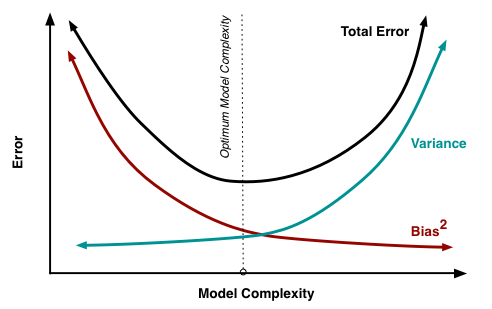
\includegraphics[ width=0.5\textwidth]{BiasVariance}
	\caption[Bias-Varianza trade-off]{\textit{Bias-Varianza trade-off}}
   \label{fig:bvtrd}
\end{figure}

\section[Tecniche selezione class.]{Model selection,Model evaluation,algorithm selection}
Il workflow nella creazione di un classificatore che funga da predittore per un problema di classificazione supervisionato è tipicamente il seguente:
\begin{description}
\item[\textbf{Algorithm selection}] E' necessario scegliere il modello\footnote{Malgrado in letteratura si parli di selezione dell'algoritmo e più corretto parlare di selezione di un modello, ad esempio in un modello come \ac{SVM} l'algoritmo l'algoritmo rappresenta la specifica tecnica risolutiva utilizzata per affrontare il problema matematico delineato da \ac{SVM}}. Spesso conoscendo pregi e difetti dei vari classificatori la selezione avviene manualmente a secondo del modello che sembra più cofacente al problema da risolvere. E' possibile tuttavia effettuare la selezione usando delle tecniche per comparare i vari modelli tra di loro per stabilire quale esibisce le migliori perfomances in base a qualche misura.
\item[\textbf{Model selection}] Con l'intento di migliorare le perfomances di generalizzazione è necessario scegliere ,a partire dal \textit{training set}, il classificatore\footnote{Malgrado in letteratura si parli di model selection è un classificatore che va selezionato.} con le migliori performances, in base a qualche misura , dallo spazio delle ipotesi. A tal fine  i modelli hanno uno o più \textit{iperparametri} cioè delle manopole da regolare.
\item[\textbf{Model evaluation}] Si vogliono stimare le performances di generalizzazione, le performances predittive (in base a qualche misura) del nostro classificatore basandoci sul \textit{test set}.
\end{description}
Per raggiungere gli obbiettivi suddetti diventa fondamentale stabilire una misura da utilizzare. Nella sezione \ref{sub:measure} vi è una breve panoramica delle misure più note che si possono adottare.

\subsection{Holdout}
Questa è una delle tecniche più semplici ma anche efficaci. Si parte dal caso semplice che si vuole fare solo model evaluation e che già si conoscono i parametri migliori e quindi non è neccessario fare model selection. Il principio ispiratore è che fare l'addestramento del classificatore e la sua valutazione sullo stesso insieme produce un'accuracy ottimisticamente biased. \textbf{Holdout} divide i campioni disponibili in un \textit{training set} e un \textit{test set} in maniera casuale di solito in maniera 2/3 1/3. Si fa l'addestramento sul \textit{training set} e poi il classificatore ottenuto viene valutato sul \textit{test set}. Infine si rieffettua l'addestramento su tutti i campioni inizialmente disponibili\footnote{Riaddestrare alla fine del processo su tutti i campioni possibili è una tecnica valida solo se si è adottata la stratificazione(vedasi \ref{stra:stra}) nello splitting dei campioni iniziali,perchè assicura che i campioni nei vari insiemi splittati restino statisticamente indipendenti}. Questo metodo ha due grandi limiti:
\begin{enumerate}
\item La suddivisone casuale dei campioni in holdout può alterare le proprietà statistiche dei campioni. Questi sono assunti essere estratti dalla stessa distribuzione di probabilità ed essere statisticamente indipendenti. Questa proprietà può venire meno: ad esempio partendo da campioni bilanciati si potrebbero generare \textit{training set} e \textit{test set} non bilanciati.
\item \label{item:holdlim} Utilizzare un numero ridotto di campioni (2/3) per effettuare l'addestramento può produrre una stima delle performances pessimisticamente biased. Si ha cioè che il classificatore non ha ancora raggiunto la sua capacità e si potrebbe apprendere un classificatore migliore utilizzando un numero di campioni più grande. 
\end{enumerate}
Il primo problema può essere superato usando una tecnica chiamata
\label{stra:stra} \textbf{stratificazione} che consiste nel suddividere l'insieme di campioni iniziale in due insiemi in modo che il bilanciamento delle classi di campioni con diverse etichette sia ancora rispettato nei risultanti sottoinsiemi. Il secondo problema invece è strutturale in quanto se si usassero tutti i campioni disponibili per l'addestramento poi si dovrebbero valutare le performances su questi stessi campioni producendo stime ottimisticamente biased. Inoltre lo scenario tipico è quello in cui si vuole fare sia model selection che model evaluation. In quest ultimo caso è necessario dividere l'insieme di campioni di partenza in (usando la stratificazione):
\begin{itemize}
\item \textbf{un training set}
\item \textbf{un validation set}
\item \textbf{un test set}
\end{itemize} 
Prima si fa model selection effettuando l'addestramento sul \textit{training set} nello spazio dei parametri. Ad esempio se si usa una tecnica come \textbf{grid-search} per ogni parametro vanno scelti i valori oppure il range in cui i valori possono variare e il passo di variazione e poi si deve effettuare l'addestramento per ogni istanza dei parametri. Alla fine ognuno di questi classificatori va valutato in base a qualche misura sui campioni del \textit{validation set} e si seleziona il modello che massimizza tale misura. Quindi in questo modo si scelgono gli iperparametri migliori. A questo punto si rieffettua l'addestramento del classificatore risultato migliore usando sia i campioni del \textit{training set} che quelli del \textit{validation set}. A questo punto si fa model evaluation, cioè il classificatore ottenuto viene valutato sul \textit{test set}. Alla fine si riaddestra su tutti i campioni inizialmente disponibili. Avendo usato in fase di model evaluation un classificatore addestrato come meno campioni(\textit{training set} e \textit{validation set}) di quelli totali è molto probabile che le misure rilevate siano delle stime pessimisticamente biased. 

\subsection{Validazione incrociata}


\section{Misure}
\label{sub:measure}
Per un problema di classificazione binaria è possibile definire la matrice di confusione come in figura \ref{fig:mco} che stabilisce le seguenti quantità numeriche per un predittore binario:
\begin{description}
\item[TP(true positive)] Campioni positivi predetti dal classificatore come positivi.
\item[TN(true negative)] Campioni negativi predetti dal classificatore come negativi.
\item[FP(false positive)] Campioni negativi predetti erroneamente dal classificatore come positivi.
\item[FN(false negative)] Campioni positivi predetti erroneamente dal classificatore come negativi.
\end{description}

\begin{figure}[htp]
	\centering
	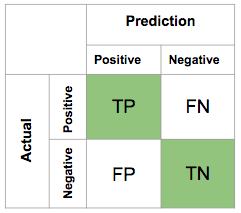
\includegraphics[ width=0.5\textwidth]{MatriceConfusione}
	\caption[Matrice di confusione]{\textit{Matrice di confusione per un problema di classificazione binaria}}
   \label{fig:mco}
\end{figure}

Allora si definisce l'\textbf{accuracy} come:
\begin{equation*}
Accuracy = \frac{TP + TN}{TP+TN+FP+FN}
\end{equation*}
e quindi indica la percentuale di campioni predetti correttamente rispetto alla totalità. Non è rilevante l'insieme su cui si definiscono la matrice di confusione e le varie misure ad esempio è possibile calcolare l'accuracy sia sul \textit{training set} che sul \textit{test set}. Inoltre è possibile calcolare la percentuale d'errore facendo:
\begin{equation*}
Errore = 1 - Accuracy
\end{equation*}
 L'accuracy però non è una misura idonea per due ragioni:
 \begin{itemize}
 \item Se l'insieme su cui si calcola l'accuracy non è bilanciato la misura d'accuracy può essere ingannevole. Ad esempio immaginiamo che il nostro classificatore sia un \textit{majority class} che predica tutti i campioni positivamente e che il \textit{test set} abbia il 90\% di campioni positivi e i restanti negativi. In questo caso avremo un'accuracy pari a 0.9 cioè del 90\% nonostante il predittore sia pessimo.
 \item Anche se l'insieme fosse bilanciato dall'accuracy non si evince se siano di più i FP oppure i FN, informazione che può essere rilevante.
 \end{itemize}
Per porre rimedio a questi problemi si usano \textbf{Precision (positive prediction value)} e \textbf{Recall (sensitivity o positive prediction value)} definite come:
\begin{alignat*}{2}
& Precision &= \frac{TP}{TP+FP}\\
& Recall &= \frac{TP}{TP+FN}
\end{alignat*}
Recall ci dice quanto è buono un classificatore a predire i campioni positivi (in quanto avendo il denominatore tutti i dati positivi dell'insieme Recall rappresenta la percentuale di campioni positivi predetta correttamente come tale). Un predittore \textit{majority class} che predice sempre i campioni come positivi (quindi FN=0) può ingannarci massimizzando Recall e rendendolo pari a 1. Precision ci dice quanti dei dati predetti come positivi sono positivi veramente; un predittore può essere ingannevole massimizzando quest'ultima misura se classifica come positivi i campioni dei quali ha una maggiore fiducia che siano positivi e negativi i restanti. Queste due misure non risultano comunque sufficienti nei casi come questo di \ac{IIR} da stringhe in cui risulta rilevante anche come vengono classificati i campioni negativi per cui si utilizzano altre due misure $Precision^{-}$(Negative prediction value) e $Recall^{-}$(Specificity o true negative rate) \cite{Bogdanov08} :
\begin{alignat*}{2}
& Precision^{-} &= \frac{TN}{TN+FN}\\
& Recall^{-} &=  \frac{TN}{TN+FP}
\end{alignat*} 
Queste ultime due misure hanno la stessa semantica di Precision e Recall ma sui campioni negativi. Si è accennato che le singole misure di per sè possono ancora essere ingannevoli tuttavia se combinate insieme tali problemi possono essere superati ad esempio se il predittore è un $majority class$ sempre positivo $Recall=1$ ma  $Recall^{-}=0$ (perchè TN=0) e quindi il problema può essere individuato. Inoltre utilizzare delle misure che combinano quelle definite sopra è necessario anche perchè per scegliere un classificatore rispetto ad un altro automaticamente è necessario avere un'unica misura. Uno dei criteri più noti e utilizzato è \textbf{F1-score (F-measure)} che effettua la media armonica tra Precisione e Recall quindi:
\begin{equation*}
\label{eq:f1s}
F1 = 2 \cdot \frac{Precision \cdot Recall}{Precision + Recall}
\end{equation*}
Questa misura può essere utilizzata il luogo dell'accuracy per insiemi non bilanciati tuttavia non fa ancora al caso nostro perchè non tiene conto dei campioni negativi che nel nostro scenario sono rilevanti. Una possibilità è quella di definire un F1-score anche sulla classe negativa usando la stessa equazione \eqref{eq:f1s} con $Precision^{-}\text{ e } Recall^{-}$ e poi mediare le due quantità tuttavia in questo scenario è più adatto e semplice utilizzare un'altra misura \textbf{MCC(Mattehws correlation coeffient)} definito come:
\begin{equation*}
MCC = \frac{TP \cdot TN−FP \cdot FN}{\sqrt{(TP+FP)(TP+FN)(TN+FP)(TN+FN)}}
 \end{equation*}
 Questa misura è ottima nel caso di dati non bilanciati e rappresenta bene la matrice di confusione ed è sicuramente più adatta di F1-score nel caso in cui sia i campioni positivi che quelli negativi sono rilevanti.